%% LaTeX2e class for student theses
%% sections/apendix.tex
%% 
%% Karlsruhe Institute of Technology
%% Institute for Program Structures and Data Organization
%% Chair for Software Design and Quality (SDQ)
%%
%% Dr.-Ing. Erik Burger
%% burger@kit.edu
%%
%% Version 1.1, 2014-11-21


\iflanguage{english}
{\chapter{Appendix}}    % english style
{\chapter{Anhang}}      % german style
\label{chap:appendix}

\section{Particle distribution around a single wire}
\label{sec:app:}
\FloatBarrier
\begin{figure}[H]
		%\centering
          \begin{subfigure}{0.49\textwidth}
                  %\flushleft
                  \scalebox{0.37}{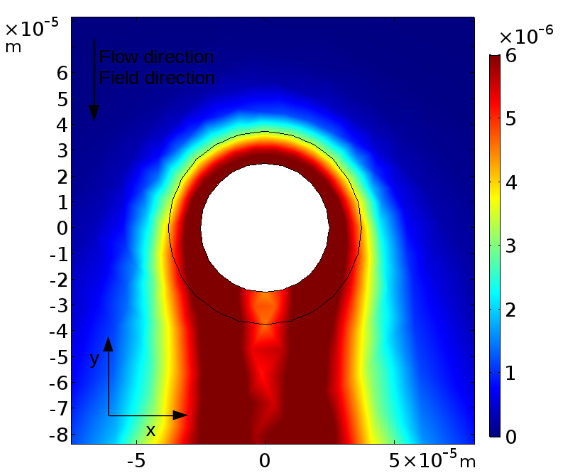
\includegraphics{figures/part_dist_wire_0mT_1.png}}
                  \caption{$B_{0}$=0\,mT}%\label{fig:hist_TruForm}
          \end{subfigure}\hfill	
	  \begin{subfigure}{0.49\textwidth}
                  %\flushleft
                  \scalebox{0.37}{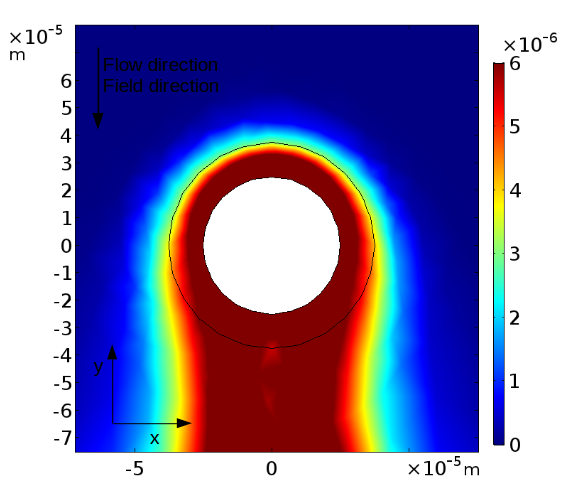
\includegraphics{figures/part_dist_wire_125mT_1.png}}
                  \caption{$B_{0}$=12.5\,mT}%\label{fig:hist_LSM}
          \end{subfigure}\hfill	\\
          \begin{subfigure}{0.49\textwidth}
                  %\flushright
                  \scalebox{0.37}{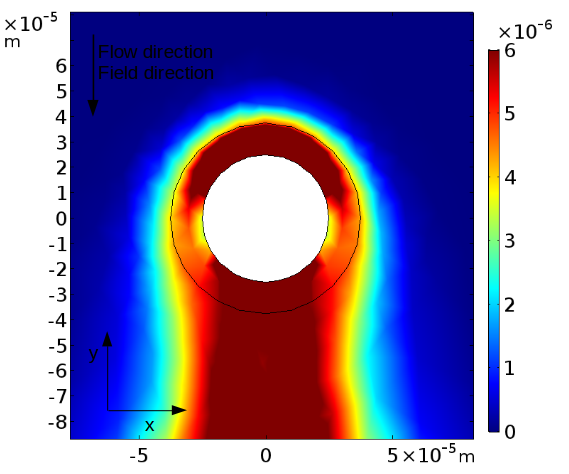
\includegraphics{figures/part_dist_wire_225mT_1.png}}
                  \caption{$B_{0}$=22.5\,mT}%\label{fig:hist_SRA}
          \end{subfigure}\hfill
        \begin{subfigure}{0.49\textwidth}
                %\flushright
                \scalebox{0.37}{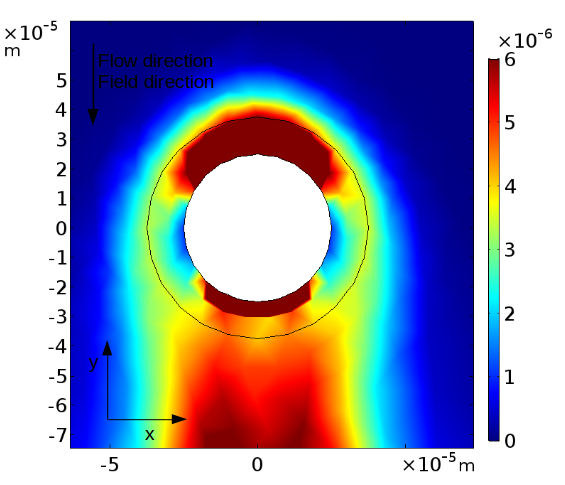
\includegraphics{figures/part_dist_wire_325mT_1.png}}
                \caption{$B_{0}$=32.5\,mT}%\label{fig:hist_SRA_sieve}
        \end{subfigure}
        \\        
        \caption[Particle distribution around a single wire for different magnetic flux densities]{Particle distribution around a single wire for four different magnetic flux densities with $R_{p}$=30\,nm, $R_{w}$=25\,\textmu m and $U_{0}$=200\,\textmu m/s where the colobar depicts the particle volume fraction $\phi$ in the fluid}
        \label{fig:Part_dist_wire}
  \end{figure}
\FloatBarrier
\section{Parameter study results for two and four wires with constant velocity boundary conditions}
\FloatBarrier
\begin{figure}[h]
		%\centering
            \begin{subfigure}{0.49\textwidth}
                  \flushleft
                  \scalebox{0.42}{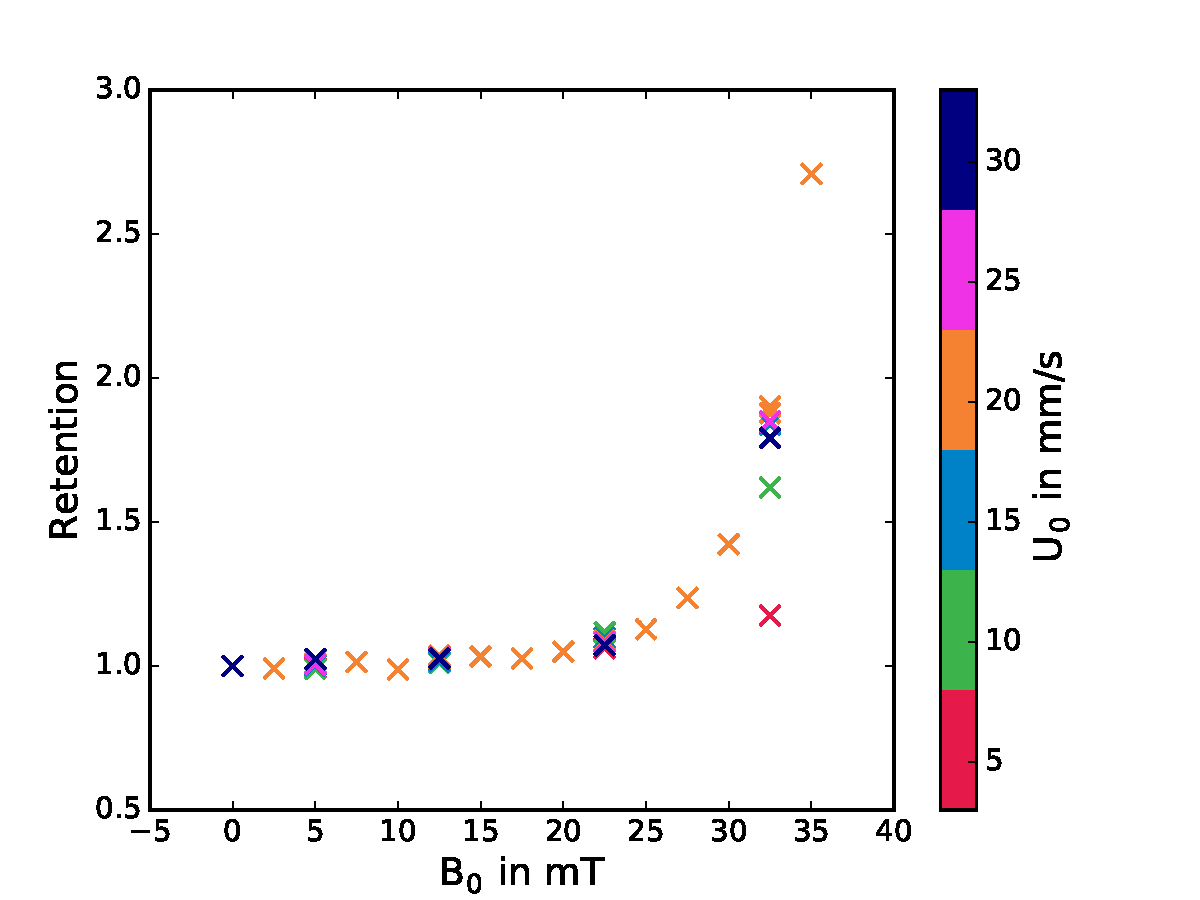
\includegraphics{figures/B0_Rp_30_U0_var_2Cylinder_constBC.pdf}}
                  \caption{Results for $R_{p}$=30\,nm and $U_{0}$ variable}\label{subfig:tw_constBC_U0_var}
          \end{subfigure}\hfill
        \begin{subfigure}{0.49\textwidth}
                \flushright
                \scalebox{0.42}{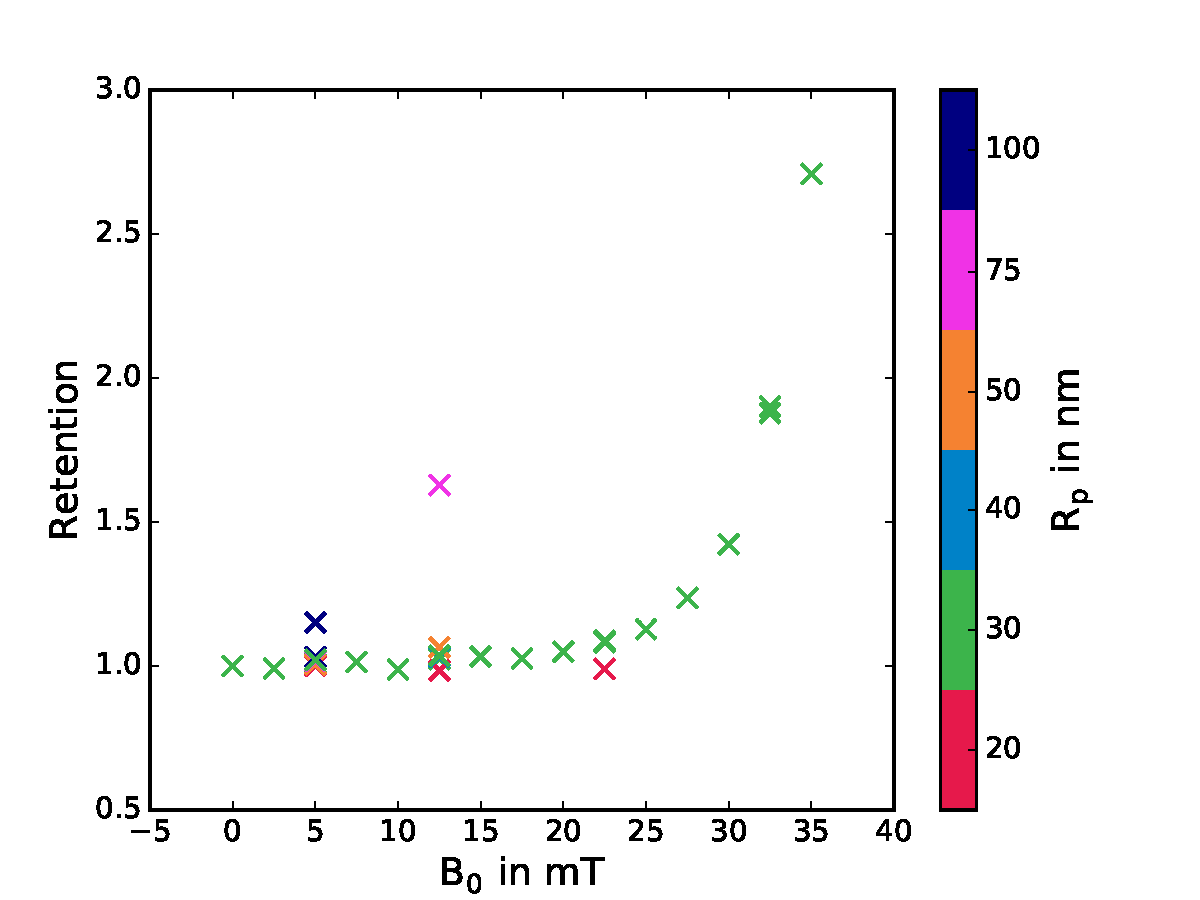
\includegraphics{figures/B0_Rp_var_U0_20_2Cylinder_constBC.pdf}}
                \caption{Results for $R_{p}$ variable and $U_{0}$=200\,\textmu m/s}\label{subfig:tw_constBC_Rp_var}
        \end{subfigure}
        \\       
          \caption[Parameter study results of the simulated retention of nanoparticles on two wires with a constant velocity boundary condition at the channel walls]{Parameter study results of the simulated retention of nanoparticles on two wires with a constant velocity boundary condition at the channel walls: the retention is plotted against the magnetic flux density $B_{0}$ in mT of the external applied magnetic field, the colorbar indicates the values of the varied parameter while the other parameters where held constant; the retention was calculated by the division of the measured residence time by the residence time for 0\,mT at the same conditions}
        \label{fig:tw_param_res_constBC}
  \end{figure}
        
\begin{figure}[h]
		%\centering
            \begin{subfigure}{0.49\textwidth}
                  \flushleft
                  \scalebox{0.42}{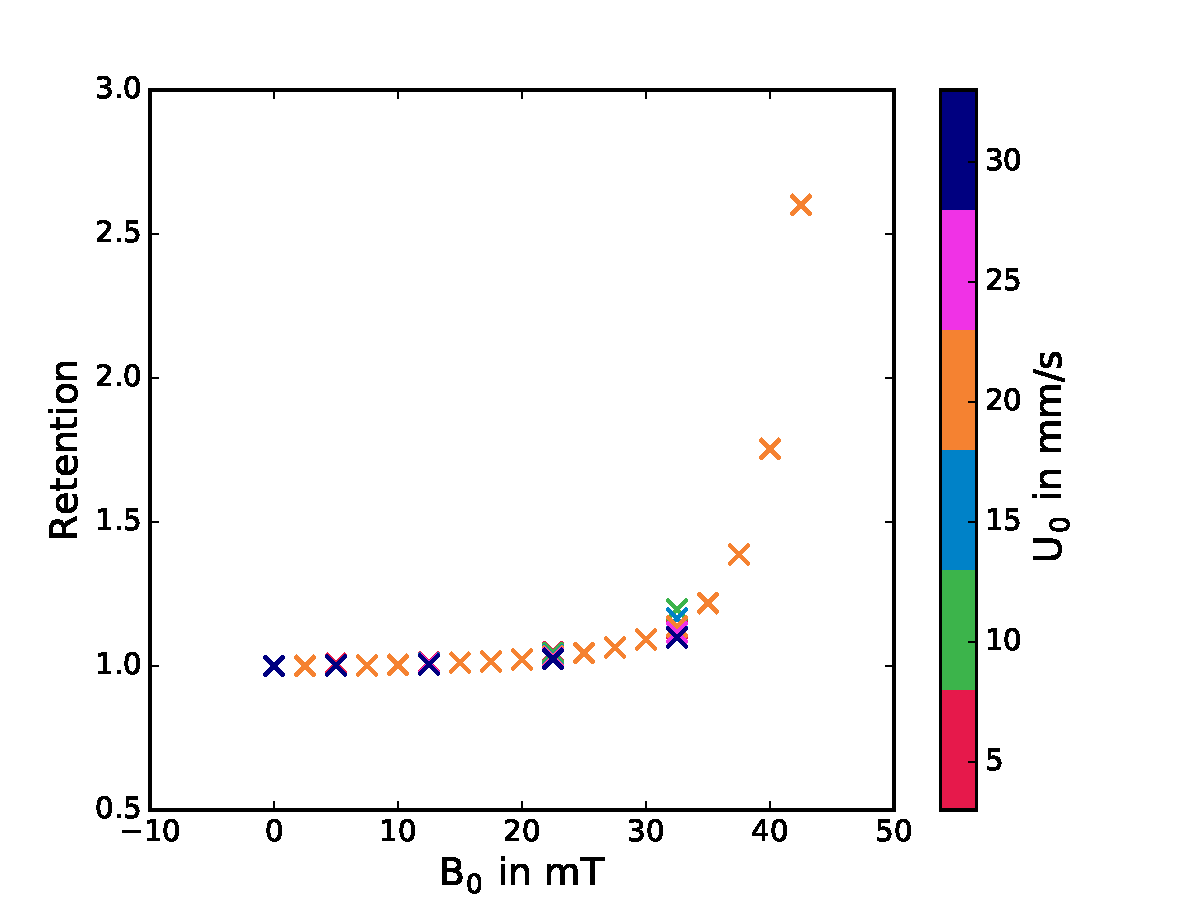
\includegraphics{figures/B0_Rp_30_U0_var_4Cylinder_constBC.pdf}}
                 \caption{Results for $R_{p}$=30\,nm and $U_{0}$ variable}\label{subfig:fw_constBC_U0_var}
          \end{subfigure}\hfill
        \begin{subfigure}{0.49\textwidth}
                \flushright
                \scalebox{0.42}{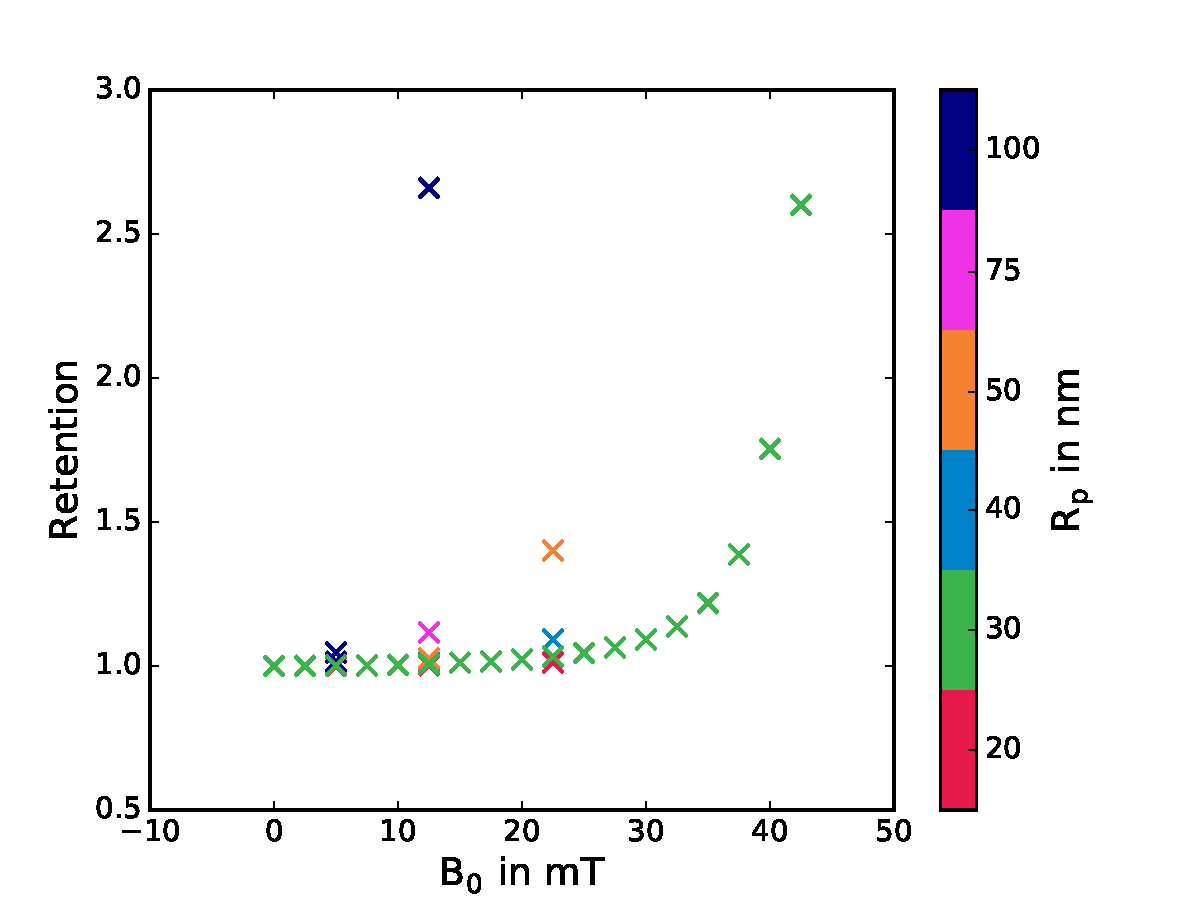
\includegraphics{figures/B0_Rp_var_U0_20_4Cylinder_constBC.pdf}}
                 \caption{Results for $R_{p}$ variable and $U_{0}$=200\,\textmu m/s}\label{subfig:fw_constBC_Rp_var}
        \end{subfigure}
        \\
        
          \caption[Parameter study results of the simulated retention of nanoparticles on four wires with a constant velocity boundary condition at the channel walls]{Parameter study results of the simulated retention of nanoparticles on four wires with a constant velocity boundary condition at the channel walls: the retention is plotted against the magnetic flux density $B_{0}$ in mT of the external applied magnetic field, the colorbar indicates the values of the varied parameter while the other parameters where held constant; the retention was calculated by the division of the measured residence time by the residence time for 0\,mT at the same conditions}
        \label{fig:fw_param_res_constBC}
  \end{figure}

\newpage
\section{Results of the retention experiments with nanoparticles of the brand Chemagen}
\FloatBarrier  
\begin{figure}[H]
        \centering
        \scalebox{0.6}{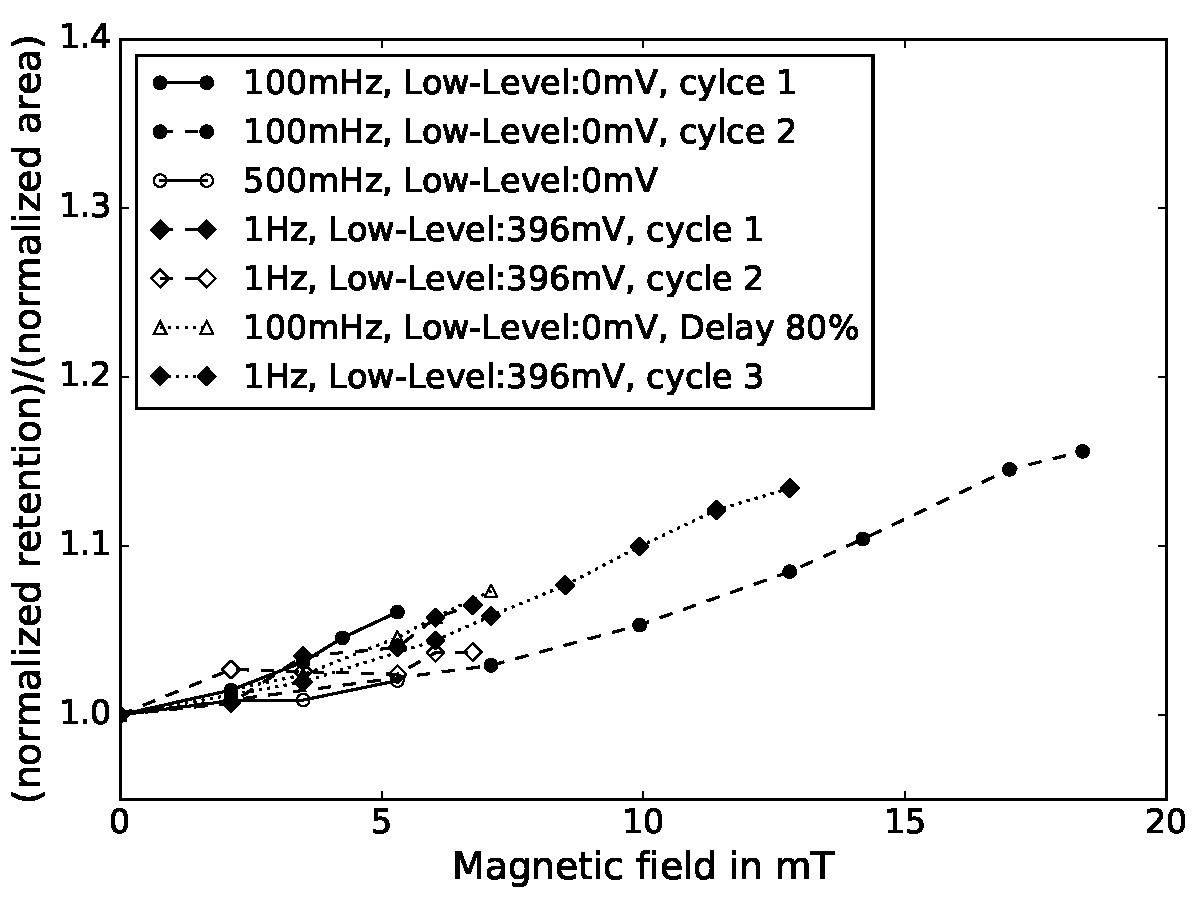
\includegraphics{figures/norm_ret_div_area_prax_comp_all.pdf}}        
        \caption[Normalized retention of Chemagen nanoparticles with the TruForm matrix material for different magnetic flux densities]{Normalized retention of Chemagen nanoparticles with the TruForm matrix material for different magnetic flux densities: The normalized retention divided by the normalized area is plotted against $B_{0}$ for magnetic fields with a frequency of 1\,Hz with a high-level value of 400\,mV and a low-level value of 396\,mV for the constant magnetic field and 0\,mV for the on/off magnetic field setting}
        \label{fig:prax_norm_ret_all}
  \end{figure}
        
\begin{figure}
		\centering
            \begin{subfigure}{0.49\textwidth}
                  \flushleft
                  \scalebox{0.42}{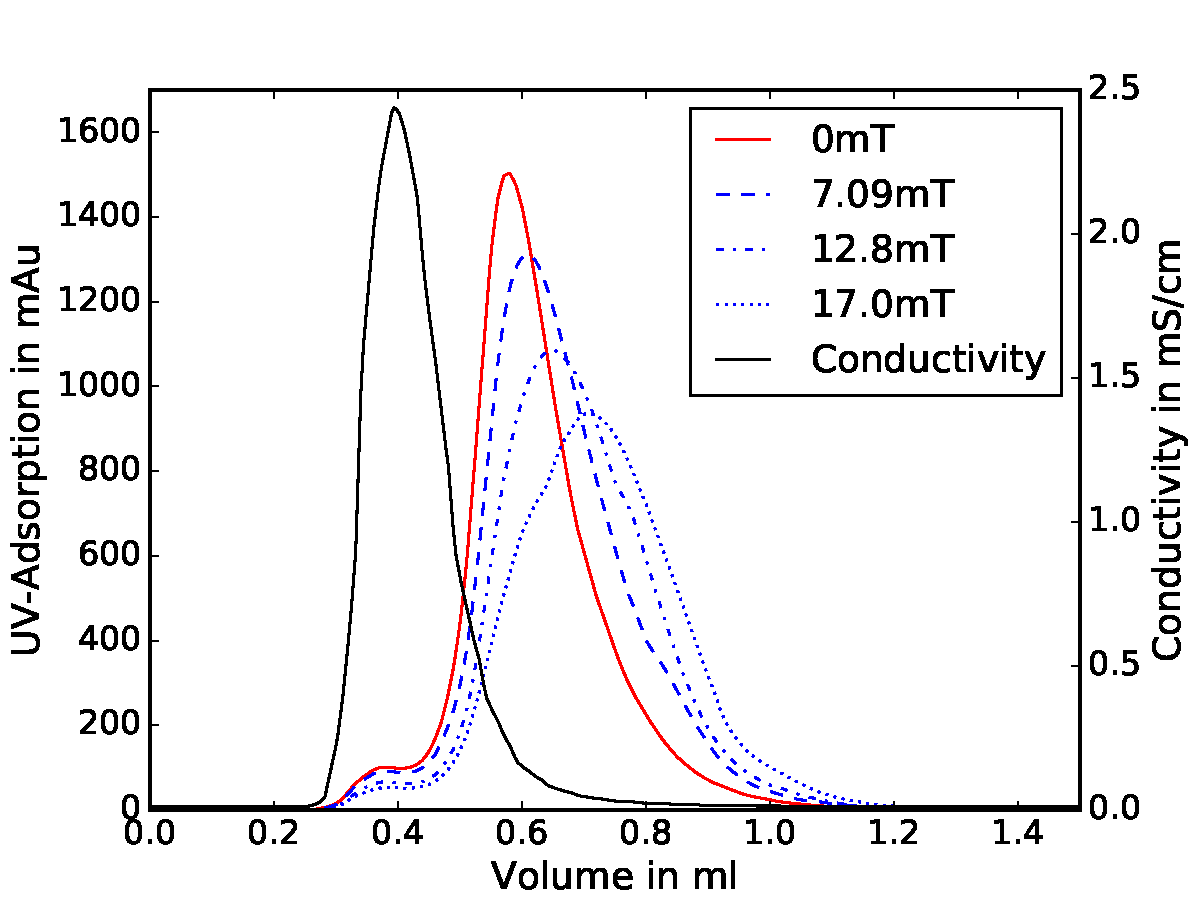
\includegraphics{figures/MF100_chemagen.pdf}}
                  \caption{Dilution 1:100}%\label{subfig:sw_periodicBC_Rw_var}
          \end{subfigure}\hfill
          \\
            \begin{subfigure}{0.49\textwidth}
                  \flushleft
                  \scalebox{0.4}{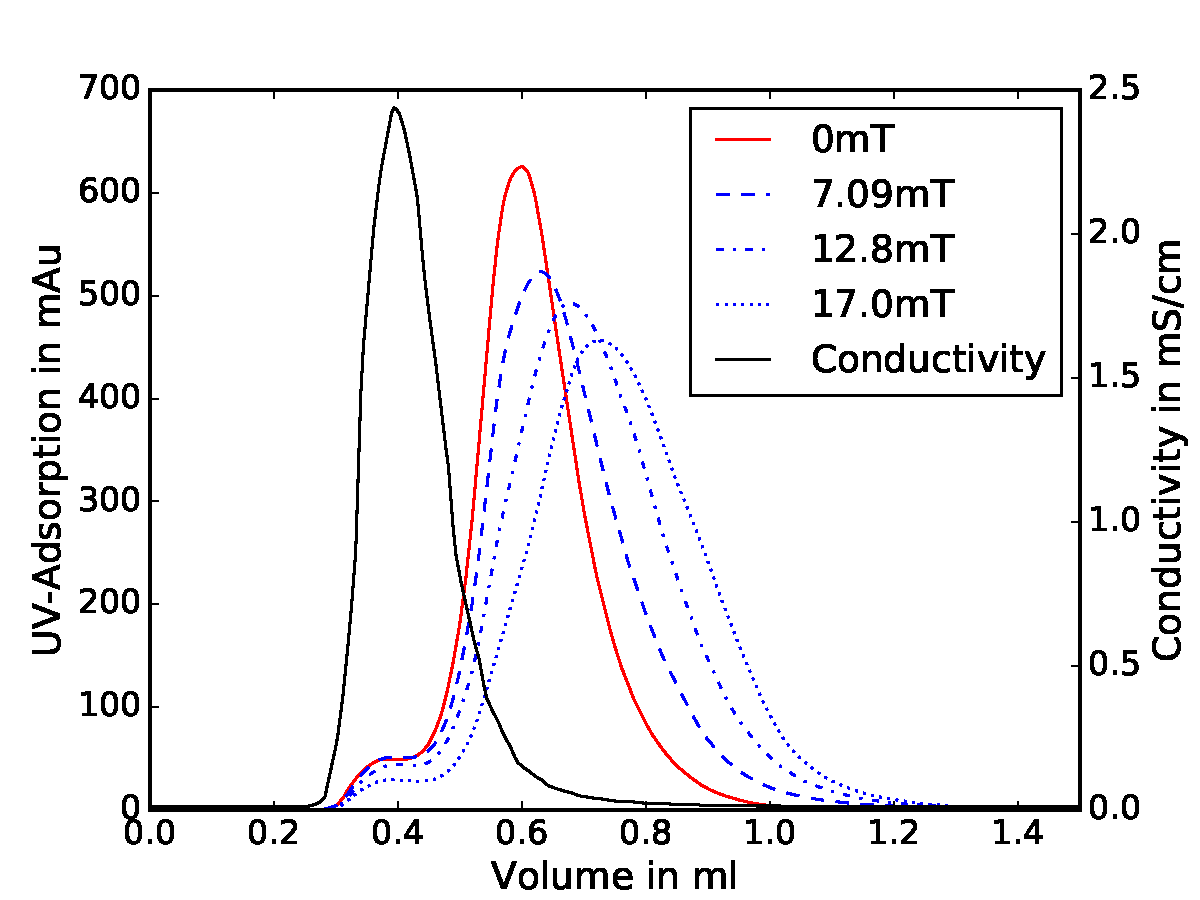
\includegraphics{figures/MF150_chemagen.pdf}}
                  \caption{Dilution 1:150}%\label{subfig:sw_periodicBC_U0_var}
          \end{subfigure}\hfill
        \begin{subfigure}{0.49\textwidth}
                \flushright
                \scalebox{0.4}{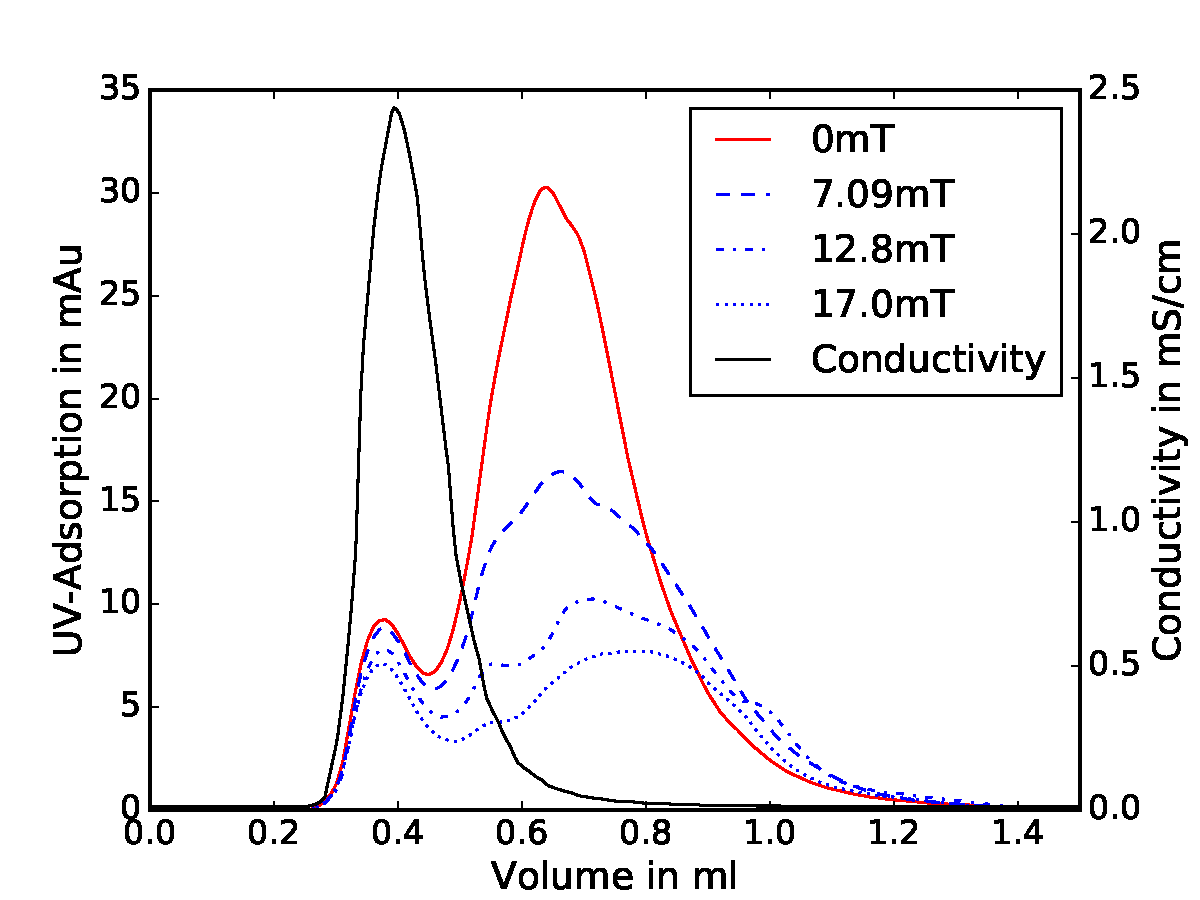
\includegraphics{figures/MF200_chemagen.pdf}}
                \caption{Dilution 1:200}%\label{subfig:sw_periodicBC_Rp_var}
        \end{subfigure}
        \\
        
        \caption[Peaks of the retention experiments conducted with different concentrations of the Chemagen nanoparticles]{Peaks of the retention experiments conducted with different concentrations of the Chemagen nanoparticles: the UV-adsorption of the nanoparticles in mAu for different magnetic fields (red and blue lines) and the conductivity (black line) in mS/cm plotted against the volume in ml }
        \label{fig:diff_conc_chemagen_peaks}
  \end{figure}        
		
\setcounter{figure}{0}
		
